\documentclass[a4paper]{article}
\usepackage[utf8]{inputenc}

% typography: load CMU fonts to get bold small caps.
\usepackage{fontspec}
%\setsansfont{CMU Sans Serif}
%\setmainfont{CMU Serif}
%\setmonofont{CMU Typewriter Text}
\usepackage{lmodern}
\usepackage{microtype}

% references
\usepackage[backend=biber]{biblatex}

\usepackage{booktabs}
\usepackage{listings}

%\usepackage{syntax}
\usepackage{amsmath}
\usepackage[super]{nth}

% illustrations
\usepackage{xcolor}
\usepackage{graphicx}
\usepackage{tikz}
\usepackage{tikz-qtree}
\usetikzlibrary{shapes,patterns,positioning,trees}

% hyperlinks
\usepackage[
  colorlinks,
  linkcolor={red!40!black},
  citecolor={blue!60!black},
  urlcolor={blue!60!black}
]{hyperref}
\usepackage{glossaries-extra}

\addbibresource{refs.bib}

\title{Filesystems}
\author{Patrick M. Elsen <pelsen@xfbs.net>}
\date{\today}

\setabbreviationstyle{long-short-sc}
\newabbreviation{fat}{fat}{File Allocation Table}
\newabbreviation{ext}{ext}{Extended File System}
\newabbreviation{ntfs}{ntfs}{New Technology File System}
\newabbreviation{uid}{uid}{User ID}
\newabbreviation{gid}{gid}{Group ID}
\newabbreviation{fifo}{fifo}{First In, First Out}
\newabbreviation{ipc}{ipc}{Interprocess Communication}
\newabbreviation{icmp}{icmp}{Internet Control Message Protocol}
\newabbreviation{acl}{acl}{Access Control Lists}
\newabbreviation{posix}{posix}{Portable Operating Systems Interface}
\newabbreviation{gui}{gui}{Guided User Interface}
\newabbreviation{sip}{sip}{System Integrity Protection}
\newabbreviation{api}{api}{Application Programming Interface}
\newabbreviation{hfs+}{hfs+}{Hiearchical File System Plus}
\newabbreviation{apfs}{apfs}{Apple File System}
\newabbreviation{ssd}{ssd}{Solid State Drive}
\newabbreviation{fuse}{fuse}{Filesystem In Userspace}
\newabbreviation{lsb}{lsb}{Linux Standard Base}
\newabbreviation{fhs}{fhs}{Filesystem Hiearchy Standard}
\newabbreviation{lfn}{lfn}{Long File Names}
\newabbreviation{usb}{usb}{Universal Serial Bus}
\newabbreviation{http}{http}{Hypertext Transfer Protocol}
\newabbreviation{tcp}{tcp}{Transmission Control Protocol}
\newabbreviation{udp}{udp}{User Datagram Protocol}
\newabbreviation{dns}{dns}{Domain Name Service}
\newabbreviation{pid}{pid}{Process ID}
\newabbreviation{url}{url}{Universal Resource Locator}
\newabbreviation{uuid}{uuid}{Universally Unique Identifier}
\makeglossaries

% don't show subsubsections in toc
\addtocontents{toc}{\setcounter{tocdepth}{2}}

\begin{document}

\maketitle

\tableofcontents

\section{Introduction}

Filesystems have always been fascinating to me. They are a kind of ubiquitous database. A lot of work goes into developing and making them work. And yet, a lot of information about them is relatively unknown. In this article, I set forth to explore some of their features.

We will look at what kinds of filesystems exist in the Linux kernel, and how they differ. We will look at the API that is presented to the user. We will also explore some advanced filesystem features and even implement our own little FS with FUSE.

All that is required for following along is a bit of experience with the Linux command line. MacOS also works, but has a slightly different set of features that are also addressed. Windows users may want to install WSL, but we will also take a look at some Windows-specific quirks.

\subsection{Tools}

This document comes with some code for utilities to work with the file system. These should be compiled and used. All command line examples in this document use these utilities rather than similarly named ones shipped with your system, unless noted otherwise. Knowledge of C and reading the code is recommended, as it showcases how the syscalls used to interact with the filesystem are used.

In order to compile and use the tools, a \emph{makefile} is provided. To compile them, ensure you have the \emph{make} tool and a modern C compiler installed (\emph{gcc} and \emph{clang} are recommended, but others should work, too). Then call the makefile with the \emph{tools} target to compile all the tools appropriate for your system.

\begin{verbatim}
$ make tools
\end{verbatim}
The tools are tested to work on Linux and macOS, and might also work on BSD systems. Not all tools work on all systems, due to differences in the functionality provided by the kernel.

% http://pages.cs.wisc.edu/~remzi/OSTEP/file-devices.pdf
% http://pages.cs.wisc.edu/~remzi/OSTEP/file-intro.pdf
% http://pages.cs.wisc.edu/~remzi/OSTEP/file-implementation.pdf
% http://pages.cs.wisc.edu/~remzi/OSTEP/file-ffs.pdf
% http://pages.cs.wisc.edu/~remzi/OSTEP/file-lfs.pdf
% http://pages.cs.wisc.edu/~remzi/OSTEP/file-journaling.pdf
% http://pages.cs.wisc.edu/~remzi/OSTEP/file-dialogue.pdf

\section{History}

UNIX as an operating system took the concept of a file system and really took it to the next level. The idea was that \emph{everything} could be a file. We see this today by some of the well-known character devices such as \verb|/dev/null| or \verb|/dev/urandom|, which we can accesses using the filesystem metaphor, but aren't files on disk in the typical sense.

DOS, the predecessor of the popular Windows operating system, had a comparatively limited concept of a file system. Initially, it did not support hierarchies, meaning that there were no folders, and file names were limited to just 11 characters. As personal computers became more powerful, this put DOS at a disadvantage, which resulted in them fixing it, but it still leaves some cruft in the Windows world. For example, Windows has no folder like UNIX’es \verb|/dev|, but device files are present in any directory.

\section{Filesystems}

Filesystems define how the structures we can work with (directories, files) and their metadata is stored on disk. As such, they are implemented in the kernel. 

The kernel provides an abstraction to work with filesystems using syscalls, which are used to interact with them. Practically, it should not matter what filesystem type is being used, but in practise there can be observable differences, such as when certain filesystems don't implement some features, or when they are slow for certain operations, due to using simpler but less efficient data structures.



Finding out what filesystem is in use can be accomplished with the \emph{stat} command.

\begin{verbatim}
$ stat -f /
  File: "/"
    ID: a34c153af3f0097e Namelen: 255     Type: ext2/ext3
Block size: 4096       Fundamental block size: 4096
Blocks: Total: 40605120   Free: 35164744   Available: 35160648
Inodes: Total: 20643840   Free: 20461918
\end{verbatim}

In this case, we learn that the filesystem in use is from the \textsc{ext} family of filesystems, with a 4K block size.

The most common filesystem used on Linux is \verb|ext4|, but there are plenty others. Filesystems supported by Linux are \verb|ext|, \verb|ext2|, \verb|ext3|, \verb|ext4|, \verb|hpfs|, \verb|iso9660|, \verb|JFS|, \verb|minix|, \verb|msdos|, \verb|ncpfs nfs|, \verb|ntfs|, \verb|proc|, \verb|Reiserfs|, \verb|smb|, \verb|sysv|, \verb|umsdos|, \verb|vfat|, \verb|XFS|, \verb|xiafs|.

If you want to learn more about filesystems and how they are actually implemented on-disk, the book \emph{Operating Systems: Three Easy Pieces} is a good start \cite{ostep}.

\subsection{Extended File System (EXT) family}

% https://de.wikipedia.org/wiki/Minix-Dateisystem

Linux Torvalds was using a machine running MINIX as he was developing the Linux kernel in 1991. To make sharing disks between his MINIX host and Linux easier, he decided to adopt MINIX's filesystem. MINIX is intended as an educational system, focussing more teaching structures and patterns of operating systems and file systems rather than usability. Hence, the \emph{minix} filesystem came with a lot of limitations, including limiting partition sizes to 64 MiB, file names to 14 (or 30 in newer versions) characters. It also does not offer any provisions for storing extended metadata and attributes.

% what is inode immutability?

The \emph{Extended File System} was quickly created in 1992 to address the limitations of the \emph{minix} filesystem. It allowed partition sizes of up to 2 GiB, and changed the file name size limit to 255 characters. This fixed some issues, but it was not enough to make Ext a viable file system. Notably, there was still no support for extended modification times metadata, and it suffered from performance issues due to using linked lists, which would over time become unsorted and fragmented\cite{ext2-doc}. 

As a result, in 1993 an alpha version of the \emph{Second Extended File System} was released. This introduced a maximum partition size of 2 TiB, along with support for extended metadata and performance improvements\cite{osdev:ext2,ext2-doc,ext2-impl}. Although newer file systems have been designed, such as Ext3 and Ext4, the Second Extended Filesystem is still preferred on flash drives as it requires fewer write operations (since it has no journal). 

Later, Ext2 was extended a few more times, leading to Ext3 in 2001 and Ext4 in 2008. The structures of Ext3 and Ext4 are based on Ext2 and add some additional options such as journaling, journal checksums, extents, online defragmentation, delayed allocations and larger directories to name but a few\cite{ext2-doc}.

Ext4 is currently the de-facto default filesystem for Linux systems, as it has been thoroughly battle-tested over the years, and offers good performance and reliability due to being a journaled filesystem. In this paper, we will take an in-depth look at all of the features offered by Ext4.

\subsection{File Allocation Table (FAT) family}

The \gls{fat} family of filesystems was designed by Microsoft in 1977. They have a lot of limitations compared to modern filesystems, but are very simple to implement, and hence \gls{fat} is still used today, for example required by the SD Consortium\cite{sd-assoc}.

% https://www.cs.drexel.edu/~jjohnson/2012-13/fall/cs370/resources/File%20Allocation%20Table.pdf

% https://www.win.tue.nl/~aeb/linux/fs/fat/fat-1.html

The \gls{fat} filesystem comes in a number of flavours, which have been developed over time and consist of extensions and fixes. Table \ref{tbl:fatfs} shows a list of the versions of \gls{fat} and their properties. The higher the cluster size, the larger the volume can be, but the more space is wasted as well.

\begin{table}[!h]
\centering\caption{FAT Filesystem Flavours}\label{tbl:fatfs}
\begin{tabular}{@{}llll@{}}
\toprule
Flavour & File names & File size & Volume size\\
\midrule
FAT8 & 6.3/9 & 8 MB &\\
FAT12 & 8.3 & 1 & 16 MiB (4 KiB cluster)\\
FAT16 & 8.3 & 1 & 2 GiB (32 KiB cluster)\\
FAT32 & 8.3 & 2 GiB & 2 TiB (32 KiB cluster)\\
\bottomrule
\end{tabular}
\end{table}


% https://en.wikipedia.org/wiki/Device_file#DOS,_TOS,_OS/2,_and_Windows

The original \gls{fat} filesystem was designed and implemented around 1977. It was used for some of Microsoft's products, and did not support sub-directories, instead storing all files in the root directory. On remnant of this time still exists in the “Windows” series of operating systems. Unlike \textsc{unix}, which puts special device files (these will be discussed later) like \verb|/dev/ttyS0|, which is used to access the serial console, into the \verb|/dev| directory, Windows has them exist in \emph{every directory on the system}. So, on Windows, every directory contains a virtual \verb|COM1| file used for reading to and from the first serial console.

\gls{fat}12 was introduced in 1980, changing the \emph{File Allocation Table} elements to be 12 bits instead of 8 like in the original \gls{fat}. It also changes the file name restrictions from 6.3 (six-characters, followed by an optional dot, followed by a three-character extension) to 8.3. \gls{fat}12 was eventually extended to support sub-directories as well.

In 1984, \gls{fat}16 was released, further increasing the size of the File Allocation Table entries to 16 bits.

\gls{fat} was changed once more to keep up with hard drive developments in 1996 to create \gls{fat}32, which allows for even larger file and volume sizes. At this time, a hack to support \gls{lfn} was also introduced, bringing file name length restrictions up to the common standard supported by more capable operating systems, which is 255 characters. This was done by hacking special directory entries holding the long file names, which are hidden from non-aware implementations.

Linux ships a whopping three different drivers for the \gls{fat} family of filesystems: the \emph{msdos}, \emph{umsdos} and \emph{vfat} drivers. The principal difference between these drivers is the amount of emulation for \textsc{unix} features they provide. As \gls{fat} has no native support for many features that are found on a standard \textsc{unix} system, such as extended attributes, fine-grained permissions, long file names, support for these has to be achieved with varying levels of hackery.

% https://en.wikipedia.org/wiki/FAT_filesystem_and_Linux

\begin{table}
\centering\caption{FAT File System Drivers in Linux}\label{tbl:fathack}
\begin{tabular}{@{}llll@{}}
\toprule
Driver & LFN & UNIX File Semantics & Notes\\
\midrule
msdos & No & No & Filenames limited to 8.3.\\
vfat & Yes & No & Windows-compatible.\\
umsdos & Yes & Yes & Can host Linux.\\
\bottomrule
\end{tabular}  
\end{table}


The \emph{msdos} driver performs no hackery at all, exposing only the bare minimum of features supported by the file system. The \emph{vfat} driver performs the same hackery that is done by current “Windows” operating systems, supporting \gls{lfn}. The \emph{umsdos} driver supports the whole range of \textsc{unix} file semantics, but at the expense of compatibility with other operating systems, storing any extra information in a hidden file labelled \verb|--LINUX-.---|.

\subsection{New Technology File System (NTFS)}

% todo explain a bit of history and features

The \gls{ntfs} is the filesystem currently used by Windows. It supports a lot of the advanced features that modern filesystems have, and even some obscure ones like \emph{alternate data streams}, which are similar to macOS's \emph{resource forks}, and are examined in Section \ref{sec:ads}

\subsection{Hierarchical File System Plus (HFS+)}

% todo explain a bit of history and features

The \gls{hfs+} is a filesystem currently used by Apple on their whole product range. It was introduced in 1998 to replace \textsc{hfs}, the predecessor that was used up until Mac OS 8.0. It supports all of the features expected from a modern filesystem, and also supports some interesting leftovers, such as \emph{resource forks}.

% documentation on format is partially in https://opensource.apple.com/source/xnu/xnu-1699.22.73/bsd/hfs/hfs_format.h

% https://filexray.com/home/

\subsection{Apple File System (APFS)}

The \gls{apfs} is a new filesystem developed by Apple and used across their product range. It is optimised for newer \gls{ssd} storage and has some unique features, such as filesystem snapshots, native full disk encryption, metadata integrity with checksums, and space sharing.

\section{File Hierachy}

In the \textsc{unix} world, the filesystem starts at the path \verb|/|. This is also called the \emph{root file system}. In this root, a number of directories typically exist, such as \verb|usr|, \verb|dev|, \verb|var|, \verb|bin|, and so forth.

\begin{verbatim}
$ ls /
bin  etc  lib64  mnt  run  tmp  boot   home 
lib  opt  root   src  usr  dev  lib32  media 
proc sbin sys   var
\end{verbatim}
Other filesystems are mounted in directories under \verb|/|. This means the root file system is actually a virtual file system; it is not one single file systems, but it is rather comprised of a number of different file systems mounted in different folders, handled by the \emph{vfs} driver in the kernel.

A hiearchical filessytem should be imagined as a tree. This is why the slash was chosen as a path separator, because it is slanted forward and signifies that whatever comes before it is higher in the hiearchy than what comes after it\footnote{There are some obscure systems that use the backslash character ‘\texttt{\textbackslash}’ as a path separator for curious historical reasons.}.
\begin{figure}[!h]
\centering
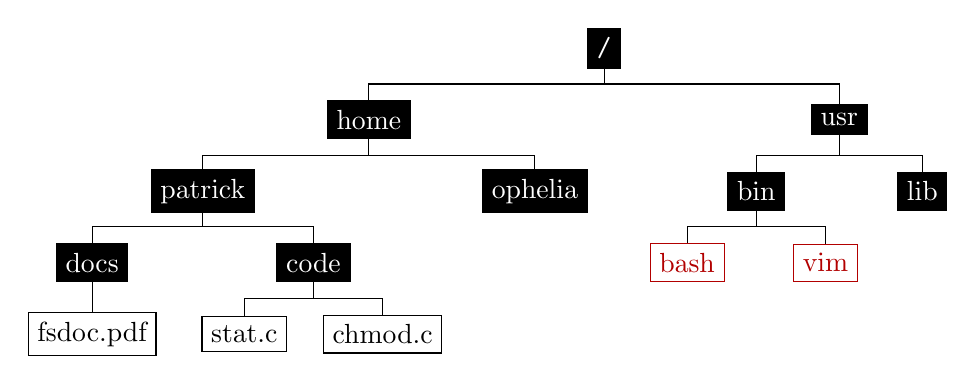
\begin{tikzpicture}[
  dir/.style={rectangle,draw,fill=black,text=white},
  file/.style={rectangle,draw},
  exe/.style={rectangle,draw=red!70!black,text=red!70!black},
  level 1/.style={sibling distance=17em,level distance=6ex},
  level 2/.style={sibling distance=5em,level distance=6ex},
]

\node [dir] {\verb|/|}
  [edge from parent fork down]
  child {node [dir] {home}
    child [sibling distance=12em] {node [dir] {patrick}
      child [sibling distance=8em] {node [dir] {docs}
        child {node [file] {fsdoc.pdf}}
      }
      child [sibling distance=8em] {node [dir] {code}
        child [sibling distance=5em] {node [file] {stat.c}}
        child [sibling distance=5em] {node [file] {chmod.c}}
      }
    }
    child [sibling distance=12em] {node [dir] {ophelia}}
  }
  child { node [dir] {usr}
    child [sibling distance=6em] { node [dir] {bin}
      child [sibling distance=5em] {node [exe] {bash}}
      child [sibling distance=5em] {node [exe] {vim}}
    }
    child [sibling distance=6em] {node [dir] {lib}}
  };
\end{tikzpicture}
\caption{File Hiearchy Tree}\label{fig:fstree}
\end{figure}
Figure \ref{fig:fstree} shows an example of how a (minimal) filesystem could be visualised. Black nodes in this tree represent directories, white nodes regular files and red nodes executable files. The difference between these will be examined in the next section. Getting the path to a file like \verb|stat.c| is done by simply joining all the names of the nodes on the path from the root to the file, in this case \verb|/home/patrick/code/stat.c|.

\subsection{Special Paths}

\begin{table}
\centering\caption{List of Special Paths}\label{tbl:specialpaths}
\begin{tabular}{@{}ll@{}}
\toprule
Path & Description\\
\midrule
\texttt{.} & Current directory\\
\texttt{..} & Parent directory\\
\texttt{\textasciitilde} & Home directory (of current user)\\
\texttt{\textasciitilde name} & Home directory (of \emph{name})\\
\bottomrule
\end{tabular}  
\end{table}

There are some conventions regarding special paths used to navigate directory hiearchies. The directory \verb|.| refers to the current directory, so in a path like \verb|/path/to/./file|, the \verb|.| does not change the path. The \verb|..| however refers to the previous (upper) directory. Therefore, a path such as \verb|/dir/../path/to/file| is equivalent to \verb|/path/to/file|, if \verb|/dir| exists as a directory and is accessible, as it is traversed.

Another convention is the special syntax for home directories. Specifying \verb|~patrick| refers to the home directory for the user \emph{patrick}, which is \verb|/home/patrick|. Specifying \verb|~root| refers to \verb|/root|, the home directory for the \emph{root} user, which is the highest-privileged user on \textsc{unix} systems.

Table \ref{tbl:specialpaths} gives an overview of all the special paths usable in \textsc{unix} systems.

% todo: lsmount util to list mounted?

% Every entry in the file hiearchy has an \emph{inode} number associated with it, uniquely identifying the file (entry).

\subsection{Mounting}

\begin{figure}[!h]
\centering
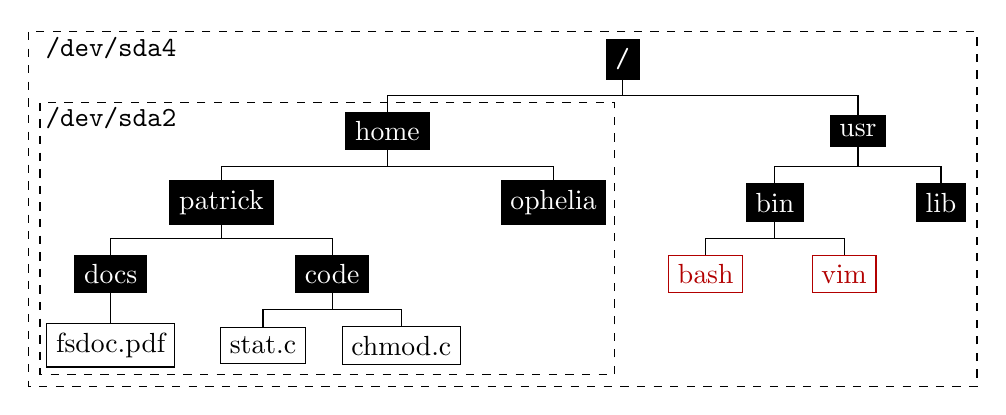
\begin{tikzpicture}[
  dir/.style={rectangle,draw,fill=black,text=white},
  file/.style={rectangle,draw},
  exe/.style={rectangle,draw=red!70!black,text=red!70!black},
  level 1/.style={sibling distance=17em,level distance=6ex},
  level 2/.style={sibling distance=5em,level distance=6ex},
]

\node [dir] {\verb|/|}
  [edge from parent fork down]
  child {node [dir] {home}
    child [sibling distance=12em] {node [dir] {patrick}
      child [sibling distance=8em] {node [dir] {docs}
        child {node [file] {fsdoc.pdf}}
      }
      child [sibling distance=8em] {node [dir] {code}
        child [sibling distance=5em] {node [file] {stat.c}}
        child [sibling distance=5em] {node [file] {chmod.c}}
      }
    }
    child [sibling distance=12em] {node [dir] {ophelia}}
  }
  child { node [dir] {usr}
    child [sibling distance=6em] { node [dir] {bin}
      child [sibling distance=5em] {node [exe] {bash}}
      child [sibling distance=5em] {node [exe] {vim}}
    }
    child [sibling distance=6em] {node [dir] {lib}}
  };
\draw[dashed,black] (-7.4,-0.55) rectangle (-0.1,-4);
\node at (-6.5,-0.75) {\verb|/dev/sda2|};
\draw[dashed,black] (-7.55,0.35) rectangle (4.5,-4.15);
\node at (-6.5,0.15) {\verb|/dev/sda4|};
\end{tikzpicture}
\caption{Illustration of Filesystem mounted in VFS}\label{fig:vfs}
\end{figure}

Mounting is the process of attaching a (real) filesystem to the virtual filesystem tree. This is typically done automatically at boot, by reading the \verb|/etc/fstab| file, which contains a list of filesystems and where and how they should be mounted. This file might look something like this.

\begin{verbatim}
LABEL=rootfs    /               ext4    defaults        0 0
LABEL=home      /home           ext4    defaults        0 0
LABEL=UEFI      /boot/efi       vfat    defaults        0 0
\end{verbatim}
At runtime, filesystems can also be dynamically mounted and unmounted. This can happen automatically, some systems exist to automount plugged-in drives, but it can also be done manually. The kernel offers the \verb|mount()| and \verb|unmount()| syscalls for this purpose.

Figure \ref{fig:vfs} shows what a filesystem mounted in another filesystem might look like. \verb|/dev/sda2| and \verb|/dev/sda4| represent two partitions on a large \gls{ssd} drive. One of them is mounted as the root file system and holds the system files, whereas the other one is mounted under \verb|/home| and holds only the user's home directories. This shows how it is possible to have a single, unified virtual filesystem, but not every file in the virtual filesystem residing on the same physical filesystem.

\subsection{Changing Filesystem Root}

The kernel offers the \verb|chroot()| syscall to change the root of the (virtual) filesystem to another folder. This is useful mostly for two reasons. At boot time, the kernel mounts the filesystem into a folder, and then changes into it. The other time this can be useful is as a security precaution: programs can be run in something called a \emph{chroot jail}, which prevents them from accessing any important system files and devices. However, this latter use has been largely replaced by the more-powerful \emph{cgroups} feature, which lets the Kernel fully isolate processes from a system.

\subsection{Filesystem Hiearchy Standard}

There is a standard for file system hiearchies in Linux-like operating systems, called the \gls{fhs}. This is a document which is put forth by the \gls{lsb}, describing what Linux installations should look like filesystem-wise\cite{fhs3}. It has a mandatory directory structure, as well as some optional components. 

While this is an important document, illustrating how most Linux installations look like, not everyone sticks to these recommendations. For example, the NixOS distribution does not adhere to the \gls{fhs}, in order to provide isolation between packages\cite{vanderburg2011}. Debian, however, does follow the \gls{fhs} standard.

Figures \ref{fig:fhs1} and \ref{fig:fhs2} provide an overview of the directories required by the \gls{fhs}, and what their purpose is as described in the standard document.

\begin{figure}
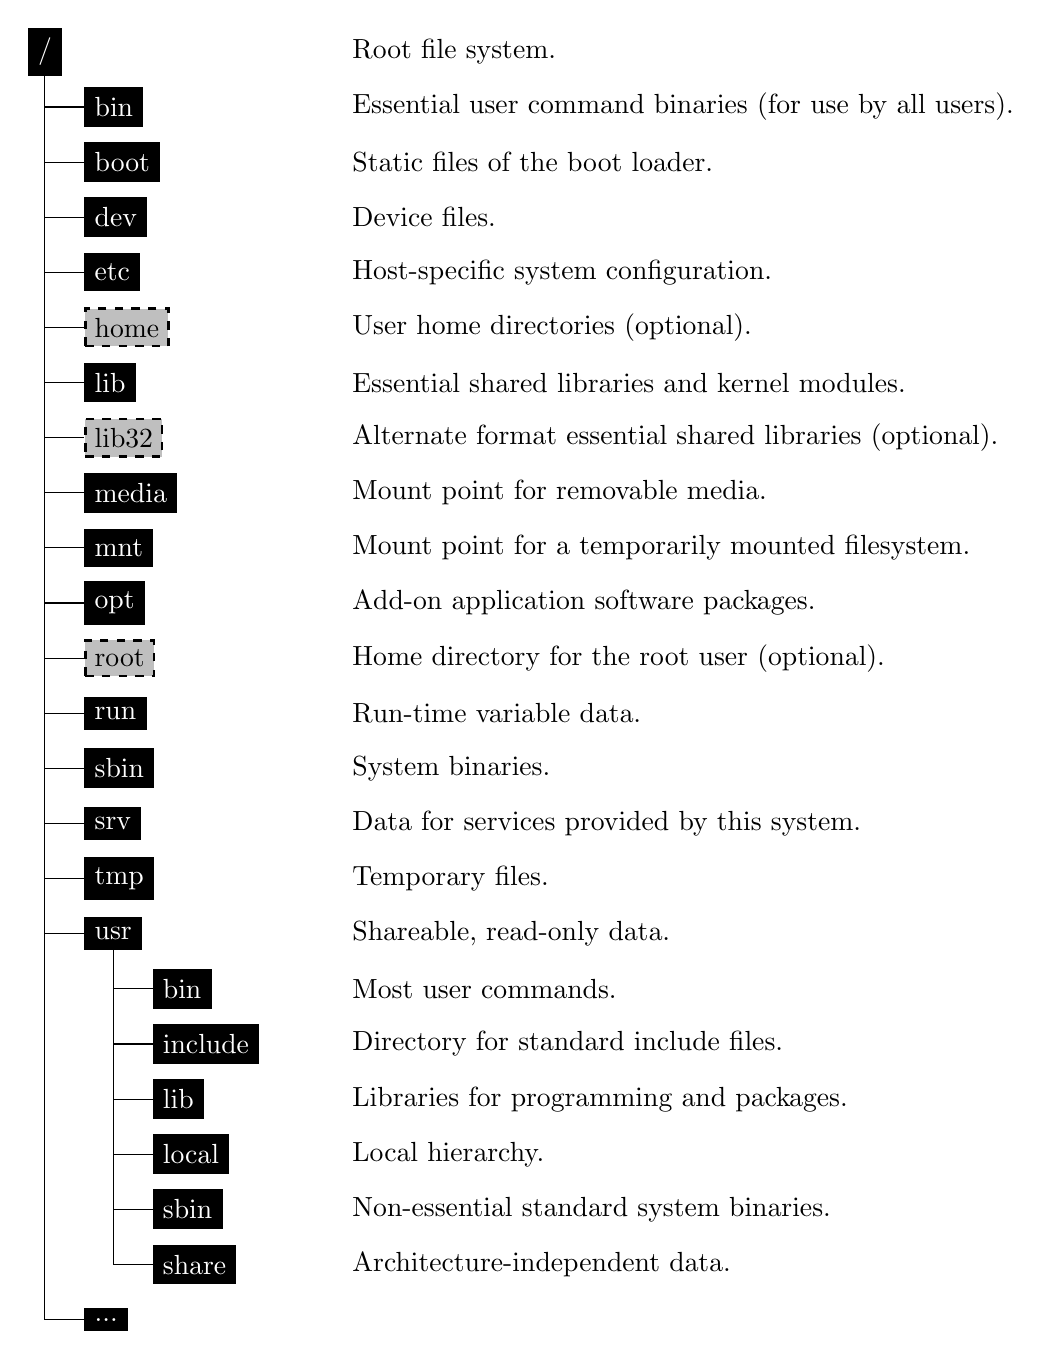
\begin{tikzpicture}[%
  dir/.style={draw=black,thick,anchor=west,draw=black,fill=black,text=white},
  opt/.style={draw=black,thick,anchor=west,dashed,fill=gray!50},
  desc/.style={anchor=west},
  grow via three points={one child at (0.5,-0.7) and
  two children at (0.5,-0.7) and (0.5,-1.4)},
  edge from parent path={(\tikzparentnode.south) |- (\tikzchildnode.west)}
]
  \node [dir] {/}
    child { node [dir] {bin}}
    child { node [dir] {boot}}
    child { node [dir] {dev}}
    child { node [dir] {etc}}
    child { node [opt] {home}}
    child { node [dir] {lib}}
    child { node [opt] {lib32}}
    child { node [dir] {media}}
    child { node [dir] {mnt}}
    child { node [dir] {opt}}
    child { node [opt] {root}}
    child { node [dir] {run}}
    child { node [dir] {sbin}}
    child { node [dir] {srv}}
    child { node [dir] {tmp}}
    child { node [dir] {usr}
      child { node [dir] {bin}}
      child { node [dir] {include}}
      child { node [dir] {lib}}
      child { node [dir] {local}}
      child { node [dir] {sbin}}
      child { node [dir] {share}}
      }
    child [missing] {}				
    child [missing] {}				
    child [missing] {}
    child [missing] {}
    child [missing] {}
    child [missing] {}
    child { node [dir] {...}};

\node at (4,    0) [desc] {Root file system.};
\node at (4, -0.7) [desc] {Essential user command binaries (for use by all users).};
\node at (4, -1.4) [desc] {Static files of the boot loader.};
\node at (4, -2.1) [desc] {Device files.};
\node at (4, -2.8) [desc] {Host-specific system configuration.};
\node at (4, -3.5) [desc] {User home directories (optional).};
\node at (4, -4.2) [desc] {Essential shared libraries and kernel modules.};
\node at (4, -4.9) [desc] {Alternate format essential shared libraries (optional).};
\node at (4, -5.6) [desc] {Mount point for removable media.};
\node at (4, -6.3) [desc] {Mount point for a temporarily mounted filesystem.};
\node at (4, -7.0) [desc] {Add-on application software packages.};
\node at (4, -7.7) [desc] {Home directory for the root user (optional).};
\node at (4, -8.4) [desc] {Run-time variable data.};
\node at (4, -9.1) [desc] {System binaries.};
\node at (4, -9.8) [desc] {Data for services provided by this system.};
\node at (4, -10.5) [desc] {Temporary files.};
\node at (4, -11.2) [desc] {Shareable, read-only data.};
\node at (4, -11.9) [desc] {Most user commands.};
\node at (4, -12.6) [desc] {Directory for standard include files.};
\node at (4, -13.3) [desc] {Libraries for programming and packages.};
\node at (4, -14.0) [desc] {Local hierarchy.};
\node at (4, -14.7) [desc] {Non-essential standard system binaries.};
\node at (4, -15.4) [desc] {Architecture-independent data.};
\end{tikzpicture}
\caption{File System Hiearchy: Example Filesystem Tree}\label{fig:fhs1}
\end{figure}

\begin{figure}
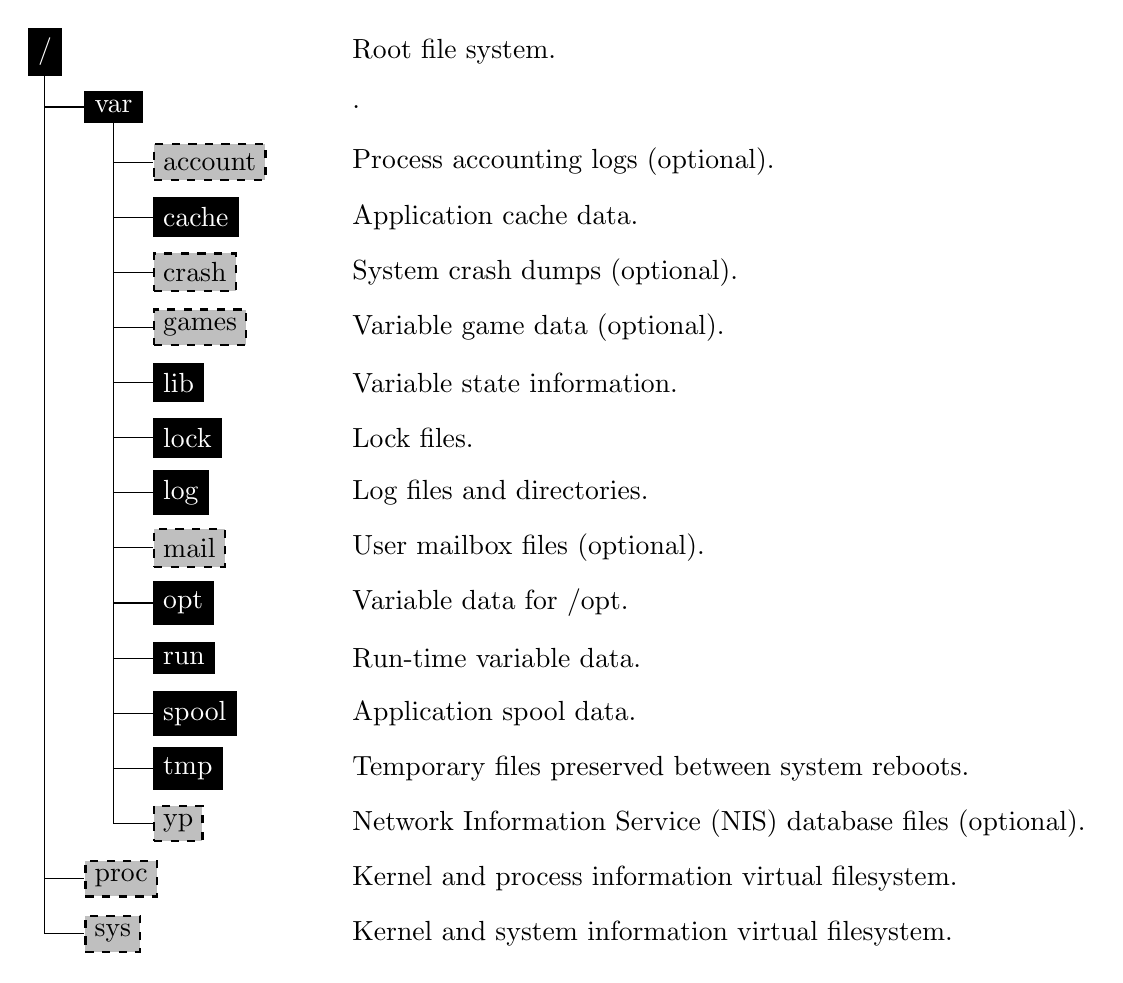
\begin{tikzpicture}[%
  dir/.style={draw=black,thick,anchor=west,draw=black,fill=black,text=white},
  opt/.style={draw=black,thick,anchor=west,dashed,fill=gray!50},
  desc/.style={anchor=west},
  grow via three points={one child at (0.5,-0.7) and
  two children at (0.5,-0.7) and (0.5,-1.4)},
  edge from parent path={(\tikzparentnode.south) |- (\tikzchildnode.west)}
]
  \node [dir] {/}
    child { node [dir] {var}
      child { node [opt] {account}}
      child { node [dir] {cache}}
      child { node [opt] {crash}}
      child { node [opt] {games}}
      child { node [dir] {lib}}
      child { node [dir] {lock}}
      child { node [dir] {log}}
      child { node [opt] {mail}}
      child { node [dir] {opt}}
      child { node [dir] {run}}
      child { node [dir] {spool}}
      child { node [dir] {tmp}}
      child { node [opt] {yp}}
      }
    child [missing] {}				
    child [missing] {}				
    child [missing] {}
    child [missing] {}
    child [missing] {}
    child [missing] {}
    child [missing] {}
    child [missing] {}
    child [missing] {}
    child [missing] {}
    child [missing] {}
    child [missing] {}
    child [missing] {}
    child { node [opt] {proc}}
    child { node [opt] {sys}};

\node at (4,    0) [desc] {Root file system.};
\node at (4, -0.7) [desc] {.};
\node at (4, -1.4) [desc] {Process accounting logs (optional).};
\node at (4, -2.1) [desc] {Application cache data.};
\node at (4, -2.8) [desc] {System crash dumps (optional).};
\node at (4, -3.5) [desc] {Variable game data (optional).};
\node at (4, -4.2) [desc] {Variable state information.};
\node at (4, -4.9) [desc] {Lock files.};
\node at (4, -5.6) [desc] {Log files and directories.};
\node at (4, -6.3) [desc] {User mailbox files (optional).};
\node at (4, -7.0) [desc] {Variable data for /opt.};
\node at (4, -7.7) [desc] {Run-time variable data.};
\node at (4, -8.4) [desc] {Application spool data.};
\node at (4, -9.1) [desc] {Temporary files preserved between system reboots.};
\node at (4, -9.8) [desc] {Network Information Service (NIS) database files (optional).};
\node at (4, -10.5) [desc] {Kernel and process information virtual filesystem.};
\node at (4, -11.2) [desc] {Kernel and system information virtual filesystem.};
\end{tikzpicture}
\caption{File System Hiearchy: Example Filesystem Tree, continued.}\label{fig:fhs2}
\end{figure}

\section{Entries}

A filesystem contains \emph{entries}. These are identified by the end user by a path such as \verb|/usr/local/bin/ruby|, where \verb|usr|, \verb|local| and \verb|bin| are \emph{directories} which form a hiearchy, and \verb|ruby| is a file. 

To the kernel, indidividual entries are identified by their \emph{inode} number, which typically is a 64-bit number. Every path (such as \verb|/usr/local/bin/ruby|), if it exists in the filesystem, resolved to an entry with an inode number. There can be multiple paths that have the same inode number. In that case, both paths refer to the same file, this is also known as a \emph{hard link}. Not all filesystems support hard links, notable \gls{apfs} does not support it.

% TODO insert citation about apfs and time machine.

It is possible to query the kernel for information (metadata) about an entry using the \verb|stat()| syscall. This returns a wealth of information, such as creation and access times, the inode number, and the entry type\footnote{For more information on this sycall, check \texttt{man 7 inode} and \texttt{man 2 stat}.}. 

In this project there is a utility, also called \verb|stat|, which uses this syscall and returns all information returned by the kernel. The output from calling this utility on \verb|~/.bashrc| looks like this.

\begin{verbatim}
$ stat ~/.bashrc
inode: 18785118
type:  regular
mode:  0644 (-rw-r--r--)
owner: 501 (pelsen)
group: 20 (staff)
links: 1
size:  17
atime: 2019-05-01T12:49:48Z
mtime: 2019-05-01T12:49:48Z
ctime: 2019-05-01T12:49:48Z
birth: 2019-05-01T12:49:48Z
dev:   1,4
rdev:  0,0
gen:   0
flags: 00000000 ()
\end{verbatim}
From the output of this utility we learn that the inode number of this particular file is 18785118. This is meaningful only to the filesystem. The type of this file is reported as a regular file. There exist a few special inode numbers, at least on \gls{ext} family filesystems\footnote{\gls{hfs+} is also confirmed to use inode number 2 for the root directory}: the root directory of a filesystem always has inode number 2. Inode number 0 is used internally, and inode 1 is a marker that a block is bad\cite{ext4-inodes}.

% https://ext4.wiki.kernel.org/index.php/Ext4_Disk_Layout#Special_inodes
% https://unix.stackexchange.com/questions/198673/why-does-have-the-inode-2

The permissions of this file are reported as 0644, this will be explored further in section \ref{sec:permissions} on page \pageref{sec:permissions}. Every entry also has an owner and a group associated with it. In this case, the file is owned by me, \gls{uid} 501.

The kernel reports how many (hard) links exist to this file. A file on the file system will have at least one link. It is possible, in Linux, to read from a file that has no links: a file is only fully removed when there are no links (entries in the filesystem to it) remain and it is not opened by any process anymore. It is thus possible to open and work with a file while another process deletes it. The behaviour here depends on the operating system, the “Windows” operating system for example does not support deleting files while they are opened by some process.

The size that is reported by the kernel is the file size in bytes. In the case of a regular file, it measures the length of data that is stored in the file.

The kernel reports four distinct times for this file. These are, in order of appearance, the \emph{access}, \emph{modification}, \emph{change}, and \emph{birth} times. The access time denotes the last time the file was accessed. On many systems, keeping track of this is disabled to reduce disk I/O and improve the longevity of hard drives. The modification time records the last time the contents of the file have been changed, such as by writing to it. The change time records the last time the file's status has changed, such as by changing its name or permissions. Lastly, the birth time records the time when the file was created. The Linux kernel does not support keeping track of the birth time.

% birth time seems to be a macOS-only feature?

% https://unix.stackexchange.com/questions/92816/can-a-file-be-retrieved-by-its-inode

\subsection{Directory}

A directory contains other entries. The syscalls used to create delete directories are \verb|mkdir()| and \verb|rmdir()|\footnote{See \texttt{man 2 mkdir} and \texttt{man 2 rmdir} for more information on these.}. This project contains the \verb|mkdir| and \verb|rmdir| tools to use these syscalls to create and delete directories.

\begin{verbatim}
$ mkdir folder 644
$ rmdir folder  
\end{verbatim}
The number 644 that is passed to the utility is the permissions of the directory, this will be discussed in the next section. 

Note that a directory may only be deleted if it is empty. Calling \verb|rmdir| on a non-empty directory results in an error.

% create touch/mkfile tool?

\begin{verbatim}
$ mkdir folder 644
$ mkfile folder/file 644
$ rmdir folder
rmdir: failed to remove 'folder/': Directory not empty
\end{verbatim}
Historically in UNIX, it was possible to use the \verb|open()| and \verb|read()| syscalls to open directories and read the list of files directly from the raw filesystem, as they were stored in a simple-to-parse format. However, with modern filesystems, this does not make sense anymore and is thus not allowed anymore, at least on Linux and on macOS.

% https://stackoverflow.com/questions/17618472/using-read-system-call-on-a-directory

The syscalls used to read directory contents are \verb|opendir()|, \verb|readdir()|, \verb|rewinddir()|, \verb|seekdir()|, \verb|telldir()|, \verb|scandir()|, and on Linux the newer \verb|getdents|. There is a tool included to use these syscalls to list a directory's contents.

\begin{verbatim}
$ mkdir dir 755
$ touch dir/file
$ lsdir
file
.
..
\end{verbatim}
The directory contents are returned in no particular order. Here you can also see the special files discussed earlier: the ‘\texttt{.}’ and ‘\texttt{..}’ relative paths, which are always returned when enumerating directory contents.

\subsection{Regular File}

Regular files are what we think of when we think of files. They contain data, and can be written to and read from. They are reported by the \verb|stat| tool as \emph{regular}.

\begin{table}
\renewcommand{\arraystretch}{1.25}
\centering\caption{List of Flags for the Open Syscall}\label{tbl:oflags}
\begin{tabular}{@{}p{2cm}p{7.5cm}p{1.5cm}@{}}
\toprule
Name & Description & Notes\\
\midrule
\verb|O_RDONLY|
& Open file as read-only.
&\\
\verb|O_WRONLY|
& Open file as write-only.
&\\
\verb|O_RDWR|
& Open file for reading and writing.
&\\
\verb|O_NONBLOCK|, \verb|O_NDELAY|
& When possible, the file is opened in non-blocking mode, meaning that operations on the file will not cause the process to wait.
&\\
\verb|O_APPEND|
& Open file in append-only mode for writing.
&\\
\verb|O_CREAT|
& Create the file (if it doesn't exist).
&\\
\verb|O_TRUNC|
& Set the file's length to zero.
&\\
\verb|O_EXCL|
& When creating the file, fail if it already exists.
&\\
\verb|O_NOFOLLOW|
& Fail if the given path name is a symbolic link.
&\\
\verb|O_CLOEXEC|
& Close this file descriptor on \verb|exec()|.
&\\
\verb|O_SHLOCK|
& Atomically obtain a shared lock.
& macOS\\
\verb|O_EXLOCK|
& Atomically obtain an exclusive lock.
& macOS\\
\verb|O_SYMLINK|
& Allow opening of symlinks. % what does this do?
& macOS\\
\verb|O_EVTONLY|
& Only deliver event notifications.
& macOS\\
\verb|O_ASYNC|
&
& Linux\\
\verb|O_DIRECT|
&
& Linux\\
\verb|O_DIRECTORY|
&
& Linux\\
\verb|O_DSYNC|
&
& Linux\\
\verb|O_LARGEFILE|
&
& Linux\\
\verb|O_NOATIME|
& Don't update the access time when the file is read.
& Linux\\
\verb|O_NOCTTY|
&
& Linux\\
\verb|O_PATH|
&
& Linux\\
\verb|O_SYNC|
& Write synchronously to the file, meaning that write operations only return when the data is on the disk.
& Linux\\
\verb|O_TMPFILE|
& Treat path as directory, create temporary unnamed file in this directory which is closed when the file descriptor is closed. 
& Linux\\
\bottomrule
\end{tabular}

\footnotesize
See \texttt{man 2 open} for more information on these flags.
\end{table}

Files can be created with the \verb|open()| sycall with the \verb|O_CREAT| flag, and they can be deleted with the \verb|unlink()| syscall. There is a tool, \verb|mkfile|, that can be used to create regular files, and a tool, \verb|unlink| that can be used to delete them.

\begin{verbatim}
$ mkfile file 644
$ lsdir .
file
.
..
$ unlink file
$ lsdir .
.
..
\end{verbatim}
After using the \verb|open()| syscall to open them, which returns a \emph{file descriptor} (an integer representing the open file), depending on the mode they were opened as, files can be read from and written to using the \verb|read()| and \verb|write()| syscalls, and finally closed with the \verb|close()| syscall.

\begin{verbatim}
$ echo hi > filename
$ cat filename
hi  
\end{verbatim}
Not only can regular files be opened, written to and read from this way, it also applies to a lot of other file types. There is a number of flags available for the \verb|open()| syscall, depending on the operating system. Table \ref{tbl:oflags} documents the flags available for macOS and Linux, and a rough description of what they do.

\subsection{Symbolic Link}

Symbolic links are essentially files containing paths to the real file. When opening them, they act as a proxy to the real file. Syscalls used for creating and reading symbolic links are \verb|symlink()| and \verb|readlink()|. There are utilities, \verb|mksym| and \verb|lssym| to create and read symlinks.

\begin{verbatim}
$ mkfile filename 644
$ mksym link filename
$ lsdir
filename
link
.
..
$ lssym link
filename  
\end{verbatim}
Aside from \verb|readlink()|, any operations performed on the symbolic link get redirected to whatever file it is pointing at. Note: on Linux, the permissions (which are discussed in the next section) of a symlink are entirely disregarded, whereas on macOS, they are considered when performing operations (a symlink that has no \emph{read} permission cannot be read from, even if the file that it is pointing to does have this permission).

\subsection{FIFO Queue}

\gls{fifo} queues are a type of special entry provided by the kernel. Unlike regular files, they don't store anything on disk. Rather, they are meant to be used by two processes, one process reading from it and the other writing to it. The data that is written is sent directly between these processes without being sent to disk first. Therefore, \gls{fifo} queues are a kind of \gls{ipc} mechanism.

\subsection{Socket}

Also called \textsc{unix} domain sockets, these are similar to network sockets in that they allow binding (listening for connections) and connecting, but without involving the network stack.

\subsection{Character Special File}

Character special files are entries that are handled completely by the kernel. They are identified by a pair of numbers, the minor and major number. Examples of this are \verb|/dev/null| and \verb|/dev/urandom|.

When reading or writing from them, the action that happens depends on their minor and major numbers in the kernel.

% list of minor and major device numbers
% https://www.kernel.org/doc/Documentation/admin-guide/devices.txt

\subsection{Block Device}

A block device is very similar to a character special device, in terms of how it is used and the fact that it, too, is a kind of virtual file. Block devices are also handled completely by the kernel, and are typically used as an interface to hardware. For example, \verb|/dev/sda| is a block device, and is used for communicating to the raw storage of the first hard drive attached to the system. 

The actual difference between block- and character devices lies in the kernel. Character devices are devices that communicate on a byte basis, such as serial ports, whereas block devices communicate with blocks at a time. An example for this would be a hard drive, which has a native block size of, say, four kilobytes. The kernel can request a single block at a time. Therefore, reading from it is most optimal when done blockwise.

\section{Permissions}\label{sec:permissions}

UNIX sports a very simple permissions model that is based on a bitmask. Every file has an owner (user) and a group associated with it. The permissions that can be given are \emph{read}, \emph{write} and \emph{execute} for each of the owner, the group and the world (anyone). In addition to that, there is a set of special flags that can be set on entries, which are \emph{set-user-\textsc{id}}, \emph{set-group-\textsc{id}} and the \emph{sticky bit}.

These permissions are typically either shown in octal form (such as 0755) or in text form.

\begin{table}[!h]
\centering\caption{List of Permission Bits}
\begin{tabular}{@{}llll@{}}
\toprule
Name & Constant & Octal & String\\
\midrule
Owner read    & \verb|S_IRUSR| & 0400 & \verb|-r--------|\\
Owner write   & \verb|S_IWUSR| & 0200 & \verb|--w-------|\\
Owner execute & \verb|S_IXUSR| & 0100 & \verb|---x------|\\
\midrule
Group read    & \verb|S_IRGRP| & 0040 & \verb|----r-----|\\
Group write   & \verb|S_IWGRP| & 0020 & \verb|-----w----|\\
Group execute & \verb|S_IXGRP| & 0010 & \verb|------x---|\\
\midrule
Others read   & \verb|S_IROTH| & 0004 & \verb|-------r--|\\
Others write  & \verb|S_IWOTH| & 0002 & \verb|--------w-|\\
Others execute& \verb|S_IXOTH| & 0001 & \verb|---------x|\\
\midrule
Set \gls{uid} & \verb|S_ISUID| & 4000 & \verb|---s------|\\
Set \gls{gid} & \verb|S_ISGID| & 2000 & \verb|------s---|\\
Sticky bit    & \verb|S_ISVTX| & 1000 & \verb|---------t|\\
\bottomrule  
\end{tabular}
\end{table}
Permissions can be changed for files using the \emph{chmod} utility. An example of setting full read, write and execute permissions for owner, group and world might look like such.

\begin{verbatim}
$ touch file
$ chmod 0777 file
$ ls -l file
-rwxrwxrwx 1 patrick patrick 0 Sep 26 14:25 file  
\end{verbatim}
When removing read permissions, even the owner is unable to read from it.

\begin{verbatim}
$ touch file
$ chmod 0000 file
$ cat file
cat: file: Permission denied
\end{verbatim}

\subsection{Read}

The read permission is needed to open a file in reading mode. For directories, the read permission bit is needed to enumerate the contents with \verb|opendir()| and \verb|readdir()|.

\subsection{Write}

The write permission is needed to open a file in writing mode. For directories, the write bit is needed to create new entries into it.

\subsection{Execute}

The execute bit is needed to execute files as binaries. This is needed to run native binaries, but also shell scripts with a hashbang or anything that goes through the Linux kernel binfmt handlers.

% https://ownyourbits.com/2018/05/23/the-real-power-of-linux-executables/

The execute bit has a different meaning for directories. If it is not set, it is not possible to \verb|chdir()| into a directory.

\subsection{Set UID and Set GID}

The \verb|setuid| bit are special in the sense that they change the effective \gls{uid} and \gls{gid} of the running process. Normally, when running an executable, the \gls{uid} and \gls{gid} are set to that of the user that executes it.

\begin{verbatim}
$ ./perms
uid 1000 (patrick)
gid 1000 (patrick)
euid 1000 (patrick)
egid 1000 (patrick)  
\end{verbatim}
However, when the Set \gls{uid} bit is set, then the effective \gls{uid} is set to that of the user who \emph{owns} the executable, rather than the one who runs it.

\begin{verbatim}
$ chown root perms
$ chmod u+s perms
$ ./perms
uid 1000 (patrick)
gid 1000 (patrick)
euid 0 (root)
egid 1000 (patrick)  
\end{verbatim}
This functionality is used in executables that need extra capabilities but should be usable by non-root users as well. Examples for this are the \verb|/bin/ping| utility, which needs raw access to generate \gls{icmp} ping packets, or \verb|/usr/bin/sudo|, which grants superuser rights to regular users depending on its configuration.

However, since Linux kernel version 2.2, the capabilities granted to a superuser have been split up into more finer-grained capabilities, and using extended attributes, one can grant specific capabilities to executables without having to give it full superuser rights. This is recommended, but not done by most major Linux distributions.

\subsection{Sticky bit}

The sticky bit has an effect on directories only. When set, files in the directory can be deleted or renamed only by the owner of the file, or the owner of the directory. This is used for directories like \verb|/tmp|, where anyone should be able to write into, but files should not be able to be deleted by anyone other than the user that created them.

\section{Quotas}

Quotas allow the system to limit disk usage for certain individuals, groups or, as is the case on Linux, projects. This probably originated back in the time where servers were large and expensive and shared between many users, and were supposed to prevent users from using a disproportionate amount of system resources (disk space).

\subsection{User}

\subsection{Group}

\subsection{Project}

% https://lwn.net/Articles/623835/
% http://man7.org/linux/man-pages/man8/setquota.8.html

\section{Attributes}

Attributes are flags that can be set on filesystem entries. These attributes have been added and developed over time and, as my research showed, not standardised across operating systems, although there does seem to be some semantic overlap.

\subsection{Linux Inode Flags}

Linux sports a number of attributes. Unlike macOS, where attributes are stored in a bitset that is returned with the \verb|stat()| syscall, in Linux a special \verb|ioctl()|\footnote{See \texttt{man ioctl\_iflags} and \texttt{man chattr} for more information on these. A full list of flags is available at \texttt{/usr/include/linux/fs.h}.} call has to be used to access and set them. Table \ref{tbl:iflags} lists all the known flags and what they are used for.

% man chattr
% man ioctl_iflags

\begin{table}
\renewcommand{\arraystretch}{1.25}
\centering\caption{Linux Inode Flags List}\label{tbl:iflags}
\begin{tabular}{@{}lp{8cm}@{}}
\toprule
Name & Description\\
\midrule
\verb|FS_SECRM_FL|
& Mark the file for secure deletion.  This feature is not implemented by any filesystem, since the task of securely erasing a file from a recording medium is surprisingly difficult.\\

\verb|FS_UNRM_FL|
& Allow the file to be undeleted if it is deleted.  This feature is not implemented by any filesystem, since it is possible to implement file-recovery mechanisms outside the kernel.\\

\verb|FS_COMPR_FL|
& Store the file compressed on disk. Not supported by most filesystems apart from \emph{btrfs}.\\

\verb|FS_SYNC_FL|
& Make  file updates synchronous.\\

\verb|FS_IMMUTABLE_FL|
& The file is immutable, no changes are permitted to contents or metadata. Can only be set by superuser.\\

\verb|FS_APPEND_FL|
& The file can only be opened in append mode.\\

\verb|FS_NODUMP_FL|
& Don't include this file in backups made using \emph{dump}.\\

\verb|FS_NOATIME_FL|
& Don't  update  the  file  last access time when the file is accessed.\\

\verb|FS_ENCRYPT_FL|
& Encrypted file.\\

\verb|FS_BTREE_FL|
& B-tree format dir.\\

\verb|FS_INDEX_FL|
& Hash-indexed directory.\\

\verb|FS_IMAGIC_FL|
& AFS directory.\\

\verb|FS_EXTENT_FL|
& This file uses extents.\\

\verb|FS_DIRSYNC_FL|
& Write directory changes synchronously to disk. Can be applied only to directories.\\

\verb|FS_JOURNAL_DATA_FL|
& Enable journaling of file data on \textsc{ext3} and \textsc{ext4} filesystems.\\

\verb|FS_NOCOW_FL|
& The file will not be subject to copy-on-write updates.\\

\verb|FS_NOTAIL_FL|
& This flag is supported only on Reiserfs.  It disables the Reiserfs tail-packing feature, which tries to pack small files (and the final fragment of larger files)  into  the  same  disk block as the file metadata.\\

\verb|FS_PROJINHERIT_FL|
& Inherit the quota project ID.  Files and subdirectories will inherit the project ID of the directory.\\

\verb|FS_TOPDIR_FL|
& Mark a directory for special treatment under the Orlov block-allocation strategy.\\
\bottomrule
\end{tabular}
\end{table}

The \verb|lsattr| utility included allows querying the Kernel for attributes of filesystem entries. It decodes the flags into human-readable names.

\begin{verbatim}
$ lsattr file
extent
\end{verbatim}

\subsubsection{Append-only file}

The xxx.

\subsection{MacOS Flags}

% help: what is https://ss64.com/osx/setfile.html setfile? 
% what does it do and how does it work?

% how are these flags different from attrs like getattrlist
% and setattrlist?

MacOS also supports file attributes, called \emph{flags}. They are returned as a bitmask in the \verb|sv_flags| field of the \verb|stat()| syscall. The \verb|stat| utility included in this project displays the flags set for a given file by using the system-provided \verb|fflagstostr()| function to decode the bitmaks to a comma-delimited string.

\begin{verbatim}
$ stat /bin | grep flags
flags: restricted,hidden
\end{verbatim}
Table \ref{tbl:macosflags} lists all flags currently known to and implemented in the MacOS kernel, as of the time of writing\footnote{\texttt{/Library/Developer/CommandLineTools/SDKs/MacOSX.sdk/usr/include/sys/stat.h} documents the currently known and used flags.}. Some flags (those beginning with \verb|SF_|) are limited in that they can only be set by the superuser, and while \gls{sip} is active, additional restrictions apply when setting or clearing certain flags. 
\begin{table}
\centering\caption{MacOS File Attributes (Flags)}\label{tbl:macosflags}
\begin{tabular}{@{}lllp{5cm}@{}}
\toprule
Name & Constant & Value (hex) & Description\\
\midrule
\emph{nodump} & \verb|UF_NODUMP| & 00\,00\;00\,01 & Don't dump this file.\\
\emph{uchg} & \verb|UF_IMMUTABLE| & 00\,00\;00\,02 & Immutable.\\
\emph{uappnd} & \verb|UF_APPEND| & 00\,00\;00\,04 & Append-Only.\\
\emph{opaque} & \verb|UF_OPAQUE| & 00\,00\;00\,08 & Opaque in union mount.\\
— & \verb|UF_COMPRESSED| & 00\,00\;00\,20 & Compressed.\\
— & \verb|UF_TRACKED| & 00\,00\;00\,40 & Tracked.\\
\emph{datavault} & \verb|UF_DATAVAULT| & 00\,00\;00\,80 & Entitlement required for reading.\\
\emph{hidden} & \verb|UF_HIDDEN| & 00\,00\;80\,00 & Hidden from \glsname{gui}.\\
\midrule
\emph{arch} & \verb|SF_ARCHIVED| & 00\,01\;00\,00 & Archived.\\
\emph{schg} & \verb|SF_IMMUTABLE| & 00\,02\;00\,00 & Immutable.\\
\emph{sappnd} & \verb|SF_APPEND| & 00\,04\;00\,00 & Append-Only.\\
\emph{restricted} & \verb|SF_RESTRICTED| & 00\,08\;00\,00 & File is under \glsname{sip}.\\
\emph{sunlnk} & \verb|SF_NOUNLINK| & 00\,10\;00\,00 & Undeletable.\\
\bottomrule  
\end{tabular}
\end{table}
Apple's \gls{sip} uses the \emph{restricted} flag to mark files and folders as system folders, which cannot be set or unset by anyone unless \gls{sip} is turned off.

It is possible, on macOS, to view the file attributes using \verb|ls| with the \verb|O| flag. 

\begin{verbatim}
$ ls -oOd /bin /Volumes /net /private
drwxr-xr-x+  4 root  hidden             128 Sep 25 20:11 /Volumes
drwxr-xr-x@ 37 root  restricted,hidden 1184 Jun 12 15:54 /bin
dr-xr-xr-x   2 root  hidden               1 Sep 24 09:31 /net
drwxr-xr-x   6 root  sunlnk,hidden      192 Sep 27  2018 /private  
\end{verbatim}

% https://en.wikipedia.org/wiki/File_attribute

\subsubsection{Nodump}

The \emph{nodump} flag can be set by any regular user and signals to the \emph{dump} utility, which was used for backups in old versions of \textsc{unix} and is long obsolete, that this file should not be included in the dump. This flag has no effect on file operations and is merely a signal to other applications.

\subsubsection{Immutable}

The \emph{uchg} and \emph{schg} flags disable any kind of modification from being done to a file with this flag. That includes writing to it, renaming it, and deleting it. 

\begin{verbatim}
$ flags file uchg
$ echo hi > file
-bash: file: Operation not permitted
$ echo hi | sudo tee file
tee: file: Operation not permitted
$ unlink file
file: Operation not permitted
$ flags file nouchg
$ unlink file
\end{verbatim}
While their effects are identical, the difference between these flags is that the \emph{uchg} flag can be set and cleared by the owner of the file, whereas the \emph{schg} flag can only be set and cleared by the superuser.

\begin{verbatim}
$ chflags schg file
$ echo hi > file
-bash: file: Operation not permitted
$ echo hi | sudo tee file
tee: file: Operation not permitted
$ unlink file
file: Operation not permitted
$ sudo chflags noschg file
$ unlink file
\end{verbatim}

\subsubsection{Append-Only}

The \emph{uappnd} and \emph{sappnd} flags prevent a file from being overwritten, by only letting processes open it in append mode. It also prevents the file from being deleted with \verb|unlink()|, renamed or hard links to it being created. The difference between the two is that \emph{uappnd} can be set and unset by the owner, whereas \emph{sappnd} can only be set and unset by the superuser.

\begin{verbatim}
$ touch file
$ flags file uappnd
$ echo hi > file
-bash: file: Operation not permitted
$ echo hi >> file
\end{verbatim}

\subsubsection{Opaque}

The opaque flag plays a role when using a union mount. This happens when mounting a filesystem over another filesystem such that both are visible. When setting the opaque flag on a directory, then this union property does not work for the directory.

% TODO: example of a union mount.

\subsubsection{Hidden}

The hidden flag hides files or folders that it is defined on from the GUI. 

\begin{figure}
\centering\caption{Hidden Makefile}\label{fig:macoshidden}
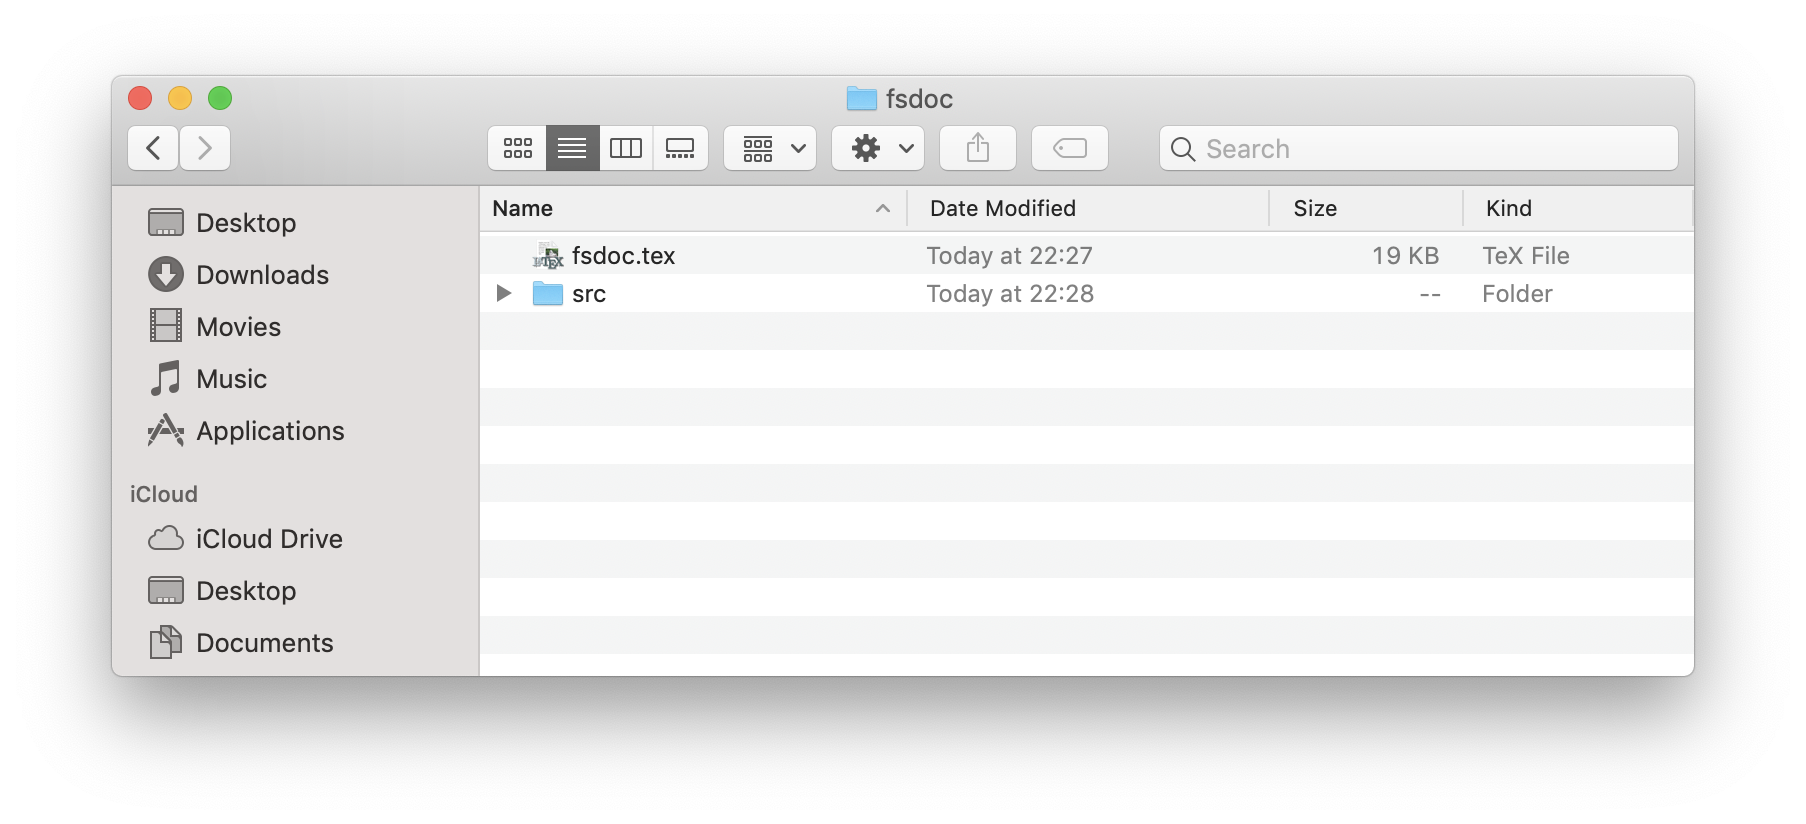
\includegraphics[width=12cm]{img/hidden}  
\end{figure}

\begin{verbatim}
$ ls
Makefile  fsdoc.tex src
$ flags Makefile hidden
$ open .
\end{verbatim}
See Figure \ref{fig:macoshidden} to see that the Makefile is indeed hidden from Finder.

\subsubsection{Archived}

The archived flag is not handled by the kernel itself. It can be set to mark that a file has been archived, such as during a backup operation. This flag has no effect on file operations.

\subsubsection{Restricted}

\subsubsection{Nounlink}

\subsubsection{Tracked}

\subsubsection{Compressed}

\subsubsection{Data Vault}

% https://mjtsai.com/blog/2018/10/25/mojave-fixes-quicklook-cache-vulnerability-with-a-datavault/
% https://unix.stackexchange.com/questions/472576/macos-mojave-directory-permissions
% https://eclecticlight.co/2018/10/25/no-entry-⛔%EF%B8%8F-access-controls-in-mojave/

Along with the \gls{sip} system, Apple has implemented the \emph{datavault} flag, which is can be set on files or folders and prevents them from being accessed (\verb|read()| or even \verb|stat()|) unless the process has \emph{entitlements}. Only system applications have these entitlements, effectively preventing anything on the system that is not audited by Apple from accessing this data.

One example of a file on which this flag is set is the QuickLook thumbnail cache\footnote{Starting with macOS 10.14.}, to prevent utilities from reading from this cache. This file is located at \texttt{/private/var/folders/\emph{xx}/\emph{yy}/C/com.apple.QuickLook.thumbnailcache}, where \emph{xx} is a two-character and \emph{yy} a 30-character random-looking token.

\begin{verbatim}
$ stat /path/to/com.apple.QuickLook.thumbnailcache
/path/to/com.apple.QuickLook.thumbnailcache: Operation not
permitted
\end{verbatim}
It is possible to list the entitlements of an executable with the \verb|codesign| utility, like such.

\begin{verbatim}
$ codesign -d --entitlements :- /Applications/Mail.app/
\end{verbatim}
These restrictions can be circumvented by turning off \gls{sip}, which can be done by booting into safe mode and using an Apple-provided command line utility, \verb|csrutil|, to disable it. Note that this potentially weakens the security of the system.

\subsubsection{Undocumented}

Not every bit in the bitfield has a name. Undocumented bits can still be set, but they have no effect. This can be used to store data. Experimenting shows that a bitmask of \verb|7F00| are bits that can be set by users that are not filtered by the system and at the same time have no effect, thus they can be used to store some information in a way that is not obvious.

\section{Extended Attributes}

Extended Attributes, often abbreviated to \emph{xattrs}, allow storing of arbitrary metadata of files on a file system. The concept of them was from the \gls{posix}\.1e draft which was withdrawn, but is still implemented on a lot of systems.

Usually, extended attributes work like a key-value store, using arbitrary strings as keys and arbitrary data as values. The amount and size of attributes that can be set depend on the filesystem. Some filesystems, such as \gls{fat}, do not support them at all, while others like the \gls{ext} family of filesystems limit them.

% https://unix.stackexchange.com/questions/489820/why-was-posix-1e-withdrawn

% https://git.kernel.org/pub/scm/linux/kernel/git/torvalds/linux.git/tree/include/uapi/linux/limits.h

\gls{posix} Extended Attributes are divided into different namespaces, with different restrictions on who and what can be set. The \emph{user} namespace has no restrictions on what attributes can be set.

\subsection{MacOS Extended Attributes}

% SetFile -type 'GSPb' -creator 'GSP+' 
% GetFileInfo -t
% GetFileInfo -c
% what do these do?

MacOS offers extended attributes that can be accessed and modified with the \verb|listxattr()|, \verb|getxattr()| and \verb|setxattr()| syscall. They are used by the system in various places, for example HFS+ Resource Forks are kept in an extended attribute named \emph{com.apple.ResourceFork}.

\begin{table}
\renewcommand{\arraystretch}{1.25}
\centering
\caption{Known Extended Attributes in MacOS}
\label{tbl:macosxattr}
\begin{tabular}{@{}p{1cm}p{10cm}@{}}
\toprule
Name & Description\\
\midrule
\texttt{com.apple.FinderInfo}\\
& 32-byte binary block of information used by Apple's Finder. The first four bytes of this are the file type, followed by the file creator. These attributes can be viewed with \verb|GetFileInfo| and set with \verb|SetFile|, and are remnants of MacOS Classic. They can also be queried with the \verb|getattrlist()| syscall.\\
\texttt{com.apple.ResourceFork}\\
& The resource fork of the file is stored internally as an extended attribute. This contains the raw data of the resource fork, which can also be accessed with \texttt{file/..namedfork/rsrc}.\\
\texttt{com.apple.lastuseddate\#PS}\\
& Binary information representing the last time it was used. Used by iCloud to offload files that are seldomly used and backed up in iCloud.\\
\texttt{com.apple.quarantine}\\
& Marker used for filed that have been downloaded.\\
\texttt{com.apple.metadata:\emph{name}}\\
& Names used by Apple to store metadata. These usually contain data in binary propery list format (see \texttt{man plist} for more information).\\
\texttt{com.apple.iwork.documentUUID\#PS}\\
& A 16-byte unique identifier for an iWork document.\\
\texttt{com.apple.icloud.desktop}\\
& \\
\texttt{com.apple.progress.fractionCompleted}\\
& Contains information about how much a task has been completed.\\
\texttt{com.apple.rootless}\\
& Marks items which are protected by \gls{sip}.\\
\bottomrule
\end{tabular}
\end{table}

% https://eclecticlight.co/2017/08/14/show-me-your-metadata-extended-attributes-in-macos-sierra/

% https://eclecticlight.co/2019/08/19/how-to-tag-documents-with-metadata-that-works-in-search/

% https://eclecticlight.co/xattred-sandstrip-xattr-tools/

\begin{table}
\centering
\caption{Known Metadata Attributes in MacOS}
\label{tbl:macosmetaattr}
\begin{tabular}{@{}lp{6cm}@{}}
\toprule
Name & Description\\
\midrule
\texttt{kMDItemWhereFroms} & Contains the \gls{url} from where a file was downloaded.\\
\texttt{kMDItemIsScreenCapture} & \\
\texttt{kMDItemScreenCaptureGlobalRect} & \\
\texttt{kMDItemScreenCaptureType} & \\
\texttt{\_kMDItemUserTags} & \\
\texttt{kMDItemDownloadedDate} & \\
\texttt{kMDLabel\_\emph{string}} & \\
\texttt{\_kTimeMachineNewestSnapshot} & Contains the oldest Time Machine backup timestamp for a major folder such as your Home folder.\\
\texttt{\_kTimeMachineNewestSnapshot} & Contains the newest Time Machine backup timestamp for a major folder.\\
\texttt{kMDItemHeadline} & Document headline\\
\texttt{kMDItemDescription} & Description of the document\\
\texttt{kMDItemCreator} & Name of the document creator, usually its author\\
\texttt{kMDItemCopyright} & Copyright notice\\
\texttt{kMDItemKeywords} &  List of keywords\\
\bottomrule
\end{tabular}
\end{table}

Table \ref{tbl:macosflags} lists some of the known extended attributes used by Apple on MacOS. For the metadata attributes, Table \ref{tbl:macosmetaattr} lists some known names. Apart from \emph{com.apple.FinderInfo}, none of these at

\subsubsection{Quarantine}

The MacOS quarantine functionality is perhaps interesting. Every file that gets downloaded is \emph{tagged} with an extended attribute named \emph{com.apple.quarantine}. This attribute contains information about the file that is used to limit what one can to with it in order to protect the system.

\begin{verbatim}
$ lsxattr com.apple.quarantine ~/Desktop/cpumemory.pdf
0081;5d32ee84;Firefox;53CAC546-3478-480D-9A2B-2FC9EAE73BA5
\end{verbatim}
The format of this tag consist of four parts, separated by semicolons. The first part is the Gatekeeper score. The higher this score, the better. The next part is a hex-encoded timestamp. This particular one decodes to 1563618948, which is 2019-07-20 12:35:48 +0200 in my local time. Finally, the last part is a \gls{uuid}, representing this file in the Gatekeeper database. If the file is an application and is launched, Gatekeeper will check if it is a known malware, and prevent it from executing if it is.

The Gatekeeper database is a regular old SQLite database that is kept at \texttt{\textasciitilde/Library/Preferences/com.apple.LaunchServices.QuarantineEventsV2}.

% https://eclecticlight.co/2019/10/03/how-has-xprotect-changed/

In addition to the Gatekeeper quarantine, Apple also has the Xprotect, which can blacklist Apps and specific versions of apps based on their certificates, outdated Internet Plugins, Safari extensions, and malware based on \textsc{yara} rules\footnote{See \url{https://yara.readthedocs.io/en/latest/} for more information on \textsc{yara}.}.

\subsection{Linux Capabilities}

We have taken a look at the setuid feature before, which lets an executable run with the \gls{uid} of it's owner rather than the person who executes it. This is mostly used to let regular users perform certain controlled tasks that are normally restricted to superusers.

However, this system has some disadvantages. Mainly that superuser privileges are very broad, and bugs occur in software. Therefore, it is best to limit the capabilities that a setuid program has to only that which it actually needs. This is to protect itself in the case in which a setuid program is exploitable, because otherwise any regular user can get full superuser privileges.

One pattern that is easy to employ for programs running as superuser is to perform the privileged action early on, such as opening a restricted file or socket, and dropping its privilege level down to that of a regular user as soon as it can. 

\begin{table}
\renewcommand{\arraystretch}{1.25}
\centering
\caption{Linux Capabilities}
\label{tbl:linuxcaps}
\begin{tabular}{@{}lp{8cm}@{}}
\toprule
Name & Description\\
\midrule
\verb|CAP_AUDIT_CONTROL| &
Enable and disable kernel auditing; change auditing filter rules; 
retrieve auditing status and filtering rules.\\

\verb|CAP_AUDIT_READ| &
Allow reading the audit log via a multicast netlink socket.\\

\verb|CAP_AUDIT_WRITE| &
Write records to kernel auditing log.\\

\verb|CAP_BLOCK_SUSPEND| &
Employ features that can block system suspend (\emph{epoll}, \texttt{EPOLLWAKEUP}, \texttt{/proc/sys/wake\_lock}).\\

\verb|CAP_CHOWN| &
Make arbitrary changes to file UIDs and GIDs.\\

\verb|CAP_DAC_OVERRIDE| &
Bypass file read, write, and execute permission checks.\\

\verb|CAP_DAC_READ_SEARCH| &
Bypass file read permission checks and directory read and execute permission checks.\\

\verb|CAP_FOWNER| &
\\

\verb|CAP_FSETID| &
\\

\verb|CAP_IPC_LOCK| &
Lock memory (\emph{mlock}, \emph{mlockall}, \emph{mmap}, \emph{shmctl})\\

\verb|CAP_IPC_OWNER| &
Bypass permission checks for operations on System V IPC objects.\\

\verb|CAP_KILL| &
Bypass permission checks for sending signals.\\

\verb|CAP_LEASE| &
Establish leases on arbitrary files.\\

\verb|CAP_LINUX_IMMUTABLE| &
Set the \verb|FS_APPEND_FL| and \verb|FS_IMMUTABLE_FL| inode flags.\\

\verb|CAP_MAC_ADMIN| &
Allow MAC configuration or state changes.\\

\verb|CAP_MAC_OVERRIDE| &
Override Mandatory Access Control (MAC).\\

\verb|CAP_MKNOD| &
Create special files using \emph{mknod}.\\

\verb|CAP_NET_ADMIN| &
\\

\verb|CAP_NET_BIND_SERVICE| &
Bind a socket to Internet domain privileged ports.\\

\verb|CAP_NET_BROADCAST| &
Make socket broadcasts, and listen to multicasts. \emph{Unused}\\

\verb|CAP_NET_RAW| &
Use RAW and PACKET sockets; bind to any address for transparent proxying.\\

\verb|CAP_SETGID| &
Make arbitrary manipulations of process GIDs and supplementary GID list; forge GID when passing socket credentials via UNIX domain sockets; write a group ID mapping in a user namespace.\\

\verb|CAP_SETFCAP| &
Set arbitrary capabilities on a file.\\

\verb|CAP_SETPCAP| &
Add any capability from the calling thread's bounding set to its inheritable set; drop capabilities from the bounding set; make changes to the \emph{securebits} flags.\\

\bottomrule
\end{tabular}
\end{table}

\begin{table}
\renewcommand{\arraystretch}{1.25}
\centering
\caption{Linux Capabilities, continued.}
\label{tbl:linuxcaps2}
\begin{tabular}{@{}lp{8cm}@{}}
\toprule
Name & Description\\
\midrule
\verb|CAP_SETUID| &
Make arbitrary manipulations of process UIDs; forge UID when passing socket credentials via UNIX domain sockets; write a user ID mapping in a user namespace.\\

\verb|CAP_SYS_ADMIN| &
\\

\verb|CAP_SYS_BOOT| &
Use \verb|reboot()| and \verb|kexec_load()|.\\

\verb|CAP_SYS_CHROOT| &
Use \verb|chroot()|.\\

\verb|CAP_SYS_MODULE| &
Load and unload kernel modules.\\

\verb|CAP_SYS_NICE| &
Change the nice value for arbitrary processes; set real-time scheduling policies for calling process, and set scheduling policies and priorities for arbitrary processes; set CPU affinity for arbitrary processes; set I/O scheduling class and priority for arbitrary processes; migrate processes to arbitrary nodes; apply \verb|move_pages()| to arbitrary processes.\\

\verb|CAP_SYS_PACCT| &
Use \verb|acct()|.\\

\verb|CAP_SYS_PTRACE| &
Trace arbitrary processes using \verb|ptrace()|; apply \verb|get_robust_list()| to arbitrary processes; transfer data to or from the memory of arbitrary processes using \verb|process_vm_readv()| and \verb|process_vm_writev()|; inspect processes using \verb|kcmp()|.\\

\verb|CAP_SYS_RAWIO| &
\\

\verb|CAP_SYS_RESOURCE| &
\\

\verb|CAP_SYS_TIME| &
Set system clock; set real-time (hardware) clock.\\

\verb|CAP_SYS_TTY_CONFIG| &
Use \verb|vhangup()|; employ various privileged \verb|ioctl()| operations on virtual terminals.\\

\verb|CAP_SYSLOG| &
Perform privileged \verb|syslog()| operations; View kernel addresses exposed via \texttt{/proc} and other interfaces when kernel pointer restrictions are enabled.\\

\verb|CAP_WAKE_ALARM| &
Trigger something that will wake up the system (such as setting timers).\\
\bottomrule
\end{tabular}
\end{table}

However, an even better approach is possible in Linux. Starting  with  kernel  2.2, Linux divides the privileges traditionally associated with superuser into distinct units, known as \emph{capabilities}, which can be independently enabled and disabled\footnote{See \texttt{man capabilities} for more information on these.}. This allows a process to only have exactly those rights which it needs — and not more, reducing potential security risks. Table \ref{tbl:linuxcaps} lists all capabilities known to the Kernel as of now.

The way this relates to filesystems is that starting with Linux version 2.6.24, it supports \emph{file capabilities}. This is similar to the setuid mechanism, however, instead of a single bit, one can specify exactly which capabilities an executable should have upon launch, rather than just which effective \gls{uid} it should take on. This information is stored in the extended attribute \emph{security.capability}.



\subsection{Access Control Lists}

\gls{acl} is a feature by which access to filesystem entries can be controlled more finely than with UNIX permissions\footnote{See \texttt{man acl} for more information}.


\section{Alternate Data Streams}\label{sec:ads}

\subsection{HFS+ Resource Fork}

A resource fork is a section of a file besides the file's actual contents that can be used to store structured data besides the unstructured data of the file itself. They appear as the extended attribute \verb|com.apple.ResourceFork|. 

Apple has a special syntax that can be used to access these forks with the standard \gls{posix} \gls{api} and tools. Given a file \verb|filename|, the special path \verb|filename/..namedforks/rsrc| can be used to access the resource fork.

\begin{verbatim}
$ touch file
$ echo hi > file/..namedforks/rsrc
$ cat file
$ cat file/..namedforks/rsrc
hi  
\end{verbatim}

Using \verb|ls -l@|, the extended attributes of the file can be listed, revealing the resource fork attribute.

\begin{verbatim}
$ ls -l@ file
-rw-r--r--@ 1 pelsen  staff  0 Sep 27 22:49 file
        com.apple.ResourceFork  3  
\end{verbatim}

These resource forks are a feature carried over from classic MacOS, and are not really used anymore. In fact, the \gls{api} to access them, \emph{Resource Manager}, have been removed. There are, to the best of my knowledge, no other named forks apart from the resource fork exposed.

\subsection{NTFS Alternate Data Streams}

% https://www.borncity.com/blog/2018/09/22/infos-zu-windows-ntfs-alternative-data-streams/

\gls{ntfs} supports alternate data streams, which are used by Microsoft to tag downloaded files as being unsafe. It is also an interesting way to hide malware.

\section{Locks}

File locking is supported with the \verb|flock()| syscall.

% TODO: example, writeup.

\section{Special Filesystems}

% TODO: introduction, comparison to /dev, justification, some history.

\subsection{Device}

% https://www.tldp.org/LDP/Linux-Filesystem-Hierarchy/html/dev.html

The device filesystem, found at \verb|/dev|, was historically not a separate filesystem but just an ordinary folder, in which special device files for the hardware could be created (with \verb|mknod|, for example). According to the \textsc{unix} \emph{everything is a file} philosophy, most of the hardware features could be accessed using the files found in the \verb|/dev| folder.

\begin{table}
\renewcommand{\arraystretch}{1.25}
\centering\caption{List of Character and Block Files In Dev Filesystem}\label{tbl:devfs}
\begin{tabular}{@{}lp{8cm}@{}}
\toprule
Name & Description\\
\midrule
\texttt{/dev/null} & Empty file. Writing to it disregards data, reading from it produces no data.\\
\texttt{/dev/zero} & File full of zeroes. Writing to it disregards data, reading from it produces infinite zeroed data.\\
\texttt{/dev/full} & Full file. Writing to it produces the error \verb|ENOSPC|, meaning \emph{no space left on device}.\\
\texttt{/dev/sda} & 
First \textsc{scsi} device (hard disk, memory sticks, external mass storage devices).\\
\texttt{/dev/sda1} & First partition on first \textsc{scsi} device.\\
\texttt{/dev/random} & Read random data from kernel (blocking).\\
\texttt{/dev/urandom} & Read random data from kernel (nonblocking, preferred).\\
\texttt{/dev/shm/} & Folder containing shared memory objects created with \verb|shm_open()|.\\
\texttt{/dev/tty0} & Current virtual console.\\
\texttt{/dev/tty} & Alias to the console (physical, virtual or pseudo device, if any) associated to the process that opens it.\\
\texttt{/dev/ttyS0} & First serial console.\\
\texttt{/dev/lp0} & First parallel port (printer, scanner).\\
\texttt{/dev/usb/} & Folder containing \gls{usb} devices.\\
\texttt{/dev/disk/} & Folder of disks by various attributes (\emph{label, uuid, path}).\\
\texttt{/dev/mem} & Raw access to system physical memory.\\
\texttt{/dev/loop0} & The first loopback device. Loopback devices are used for mounting filesystems which are not located on other block devices such as disks.\\
\texttt{/dev/stdin} & Standard input of current process. Reading from this file reads from standard input.\\
\texttt{/dev/stdout} & Standard output of current process. Writing to this file writes to standard output.\\
\bottomrule
\end{tabular}
\end{table}

% http://www.kroah.com/linux/talks/ols_2003_udev_paper/Reprint-Kroah-Hartman-OLS2003.pdf

For practical reasons, the \verb|/dev| filesystem is actually a virtual filesystem on modern Linux machines, created by the \emph{udev} driver. This \emph{udev}\footnote{See \texttt{man udev} for more information on this feature.} is a deamon that monitors the hardware, creating device files in \verb|/dev| when hardware is added or removed, and also allows for sending events to other deamons to notify them of this.

% https://www.tldp.org/LDP/sag/html/dev-fs.html
% https://unix.stackexchange.com/questions/60641/linux-difference-between-dev-console-dev-tty-and-dev-tty0/384792

On macOS, \verb|/dev| is provided by the \emph{devfs} driver, in a similar manner to Linux's \emph{udev}. The set of files provided by these two drivers is not the same, and there are differences between the kinds of special device files offered on different kernels. Table \ref{tbl:devfs} lists some common files found in the device filesystem, and what they are used for\footnote{\url{https://www.kernel.org/doc/Documentation/admin-guide/devices.txt} lists all major/minor numbers the Linux kernel supports for device files.}.

Note that special files missing in the device filesystem might still be available on a system after creating them manually. For example, the \verb|/dev/kmem| file, which is used to access the (virtual) memory of the kernel, might not exist on a typical system, but can be created easily like this.

\begin{verbatim}
$ sudo mknod -m 640 /dev/kmem c 1 2
\end{verbatim}
One interesting bit of information is that the \verb|/dev| filesystem is so ubiquitous that some applications even have some special handling for it. For example, the \emph{bash} shell, which comes as default on most Linux systems, offers special handling for paths beginning with \verb|/dev/net/tcp| and \verb|/dev/net/udp|, allowing sending of \gls{tcp} and \gls{udp} packets by writing to pseudo-files\cite{bash-redir-net} (these files don't really exist, rather writes to them are intercepted by bash and translated into socket operations).

This is an example of doing a \gls{http} request with bash redirections.

\begin{verbatim}
# open tcp connection at fd 3
exec 3<>/dev/tcp/wttr.in/80
# send http request, masquerading as curl
printf "GET / HTTP/1.0\r\n" >&3
printf "User-Agent: curl/7.58.0\r\n" >&3
printf "Host: wttr.in\r\n\r\n" >&3
# print response
cat <&3
\end{verbatim}
With the same mechanism, a \gls{dns} request can be performed over \gls{udp} with a pure bash script.

\begin{verbatim}
exec 3<>/dev/udp/9.9.9.9/53
packet="\x00\x00\x01\x00\x00\x01\x00\x00\x00\x00\x00\x00"
packet="$packet\x06github\x03com\x00\x00\x01\x00\x01"
printf $packet >&3
head -c 44 <&3 | tail -c 4 | hexdump -n 4 -e '/1 "%u" "."'
\end{verbatim}
This illustrates how powerful the everything-is-a-file metaphor is: so powerful in fact that the bash developers have decided to add virtual files that can be used to perform actions typically performed by more complicated syscalls.

% http://git.savannah.gnu.org/cgit/bash.git/tree/redir.c#n535 [cited]

\subsection{Process}

% TODO: overview, examples.

% https://www.tldp.org/LDP/Linux-Filesystem-Hierarchy/html/proc.html

% https://www.kernel.org/doc/html/latest/admin-guide/sysctl/index.html

Linux has something that other \textsc{unix}es don't have: the process filesystem, also known as \emph{procfs}. This is a virtual filesystem (meaning that the files in it are not found on a disk somewhere, but are only presented by the kernel), and can be found at the path \verb|/proc|. It's primary purpose is to let the kernel expose information about processes in a structured manner, similar to the device filesystem, which lets the kernel expose devices in a structured manner.

\begin{table}
\renewcommand{\arraystretch}{1.25}
\centering
\caption{List of Significant Files Exposed in the Process Filesystem}  
\label{tbl:procfs}
\begin{tabular}{@{}lp{8cm}@{}}
\toprule
Path & Description\\
\midrule
\texttt{/proc/apm} &
Advanced power management info.\\

\texttt{/proc/bus/} &
Directory containing bus specific information.\\

\texttt{/proc/cmdline} &
Kernel command line. \\

\texttt{/proc/cpuinfo} &
Information about the processor, such as its type, make, model, and performance.\\

\texttt{/proc/devices} &
List of device drivers configured into the currently running kernel (block and character).\\

\texttt{/proc/dma} &
Shows which DMA channels are being used at the moment.\\

\texttt{/proc/driver/} &
Various drivers grouped here, currently rtc.\\

\texttt{/proc/execdomains} &
Execdomains, related to security.\\

\texttt{/proc/fb} &
Frame Buffer devices.\\

\texttt{/proc/filesystems} &
Filesystems configured/supported into/by the kernel.\\

\texttt{/proc/fs/} &
File system parameters, currently nfs/exports.\\

\texttt{/proc/ide/} &
This subdirectory contains information about all IDE devices of which the kernel is aware.\\

\texttt{/proc/interrupts} &
Shows which interrupts are in use, and how many of each there have been.\\

\texttt{/proc/iomem} &
Memory map.\\

\texttt{/proc/ioports} &
Which I/O ports are in use at the moment.\\

\texttt{/proc/irq} &
Masks for irq to cpu affinity.\\

\texttt{/proc/isapnp} &
ISA PnP (Plug and Play) Info.\\

\texttt{/proc/kcore} &
An image of the physical memory of the system (can be ELF or A.OUT (deprecated in 2.4)). This is exactly the same size as your physical memory, but does not really take up that much memory; it is generated on the fly as programs access it. (Remember: unless you copy it elsewhere, nothing under /proc takes up any disk space at all.)\\

\texttt{/proc/kmsg} &
Messages output by the kernel. These are also routed to syslog.\\

\texttt{/proc/ksyms} &
Kernel symbol table.\\

\texttt{/proc/loadavg} &
The 'load average' of the system; three indicators of how much work the system has done during the last 1, 5 \& 15 minutes.\\
\bottomrule
\end{tabular}
\end{table}

\begin{table}
\renewcommand{\arraystretch}{1.25}
\centering
\caption{List of Significant Files Exposed in the Process Filesystem}  
\label{tbl:procfs2}
\begin{tabular}{@{}lp{8cm}@{}}
\toprule
Path & Description\\
\midrule
\texttt{/proc/locks} &
Kernel locks.\\

\texttt{/proc/meminfo} &
Information about memory usage, both physical and swap. Concatenating this file produces similar results to using 'free' or the first few lines of 'top'.\\

\texttt{/proc/misc} &
Miscellaneous pieces of information. This is for information that has no real place within the rest of the proc filesystem.\\

\texttt{/proc/modules} &
Kernel modules currently loaded. Typically its output is the same as that given by the 'lsmod' command.\\

\texttt{/proc/mounts} &
Mounted filesystems\\

\texttt{/proc/mtrr} &
Information regarding mtrrs\\

\texttt{/proc/net} &
Status information about network protocols.\\

\texttt{/proc/parport} &
Contains information about the parallel ports of your system.\\

\texttt{/proc/partitions} &
Table of partitions known to the system\\

\texttt{/proc/rtc} &
Real time clock\\

\texttt{/proc/scsi} &
Information about SCSI host adapters in the system.\\

\texttt{/proc/self} &
A symbolic link to the process directory of the program that reading it.\\

\texttt{/proc/slabinfo} &
The slabinfo file gives information about memory usage at the slab level. Linux uses slab pools for memory management above page level in version 2.2. Commonly used objects have their own slab pool (such as network buffers, directory cache, and so on).\\

\texttt{/proc/stat} &
Overall/various statistics about the system, such as the number of page faults since the system was booted.\\

\texttt{/proc/swaps} &
Swap space utilization.\\

\texttt{/proc/sys} &
This is not only a source of information, it also allows you to change parameters within the kernel without the need for recompilation or even a system reboot.\\

\texttt{/proc/tty} &
Information about the available and actually used tty's can be found in this directory. You'll find entries for drivers and line disciplines here.\\

\texttt{/proc/uptime} &
The time the system has been up.\\

\texttt{/proc/version} &
The kernel version.\\

\texttt{/proc/video} &
BTTV info of video resources.\\
\bottomrule
\end{tabular}
\end{table}

\begin{table}
\renewcommand{\arraystretch}{1.25}
\centering
\caption{List of Information on Processes exposed by the Proc Filesystem.}  
\label{tbl:procfs3}
\begin{tabular}{@{}lp{8cm}@{}}
\toprule
Path & Description\\
\midrule
\texttt{/proc/\emph{pid}/cmdline} &
Command line arguments.\\

\texttt{/proc/\emph{pid}/cpu} &
Current and last cpu in which it was executed.\\

\texttt{/proc/\emph{pid}/cwd} &
Link to the current working directory.\\

\texttt{/proc/\emph{pid}/environ} &
Values of environment variables.\\

\texttt{/proc/\emph{pid}/exe} &
Link to the executable of this process.\\

\texttt{/proc/\emph{pid}/fd} &
Directory, which contains all file descriptors.\\

\texttt{/proc/\emph{pid}/maps} &
Memory maps to executables and library files.\\

\texttt{/proc/\emph{pid}/mem} &
Memory held by this process.\\

\texttt{/proc/\emph{pid}/root} &
Link to the root directory of this process.\\

\texttt{/proc/\emph{pid}/stat} &
Process status.\\

\texttt{/proc/\emph{pid}/statm} &
Process memory status information.\\

\texttt{/proc/\emph{pid}/status} &
Process status in human readable form.\\
\bottomrule
\end{tabular}
\end{table}

Unlike the device filesystem, which contains special files that could exist on any filesystem, which have a major and a minor number to tell the kernel what device or what subsystem to communicate with, the process filesystem consists entirely of what seem to be regular files. 

The process filesystem contains a folder for every process running on the system — named after the \gls{pid} of the process, as well as some other files exposing general information from the kernel\footnote{See \texttt{man proc} for more detailed information about what information is exposed by the kernel.}. Tables \ref{tbl:procfs}, \ref{tbl:procfs2} and \ref{tbl:procfs3} list some of the files exposed in the process filesystem.

Some of the interesting features of the process filesystem include being able to read from a process's memory, by looking at \verb|/proc/<pid>/mem|. This obviously requires superuser privileges to do.

% TODO: write demo for reading mem of another process.

\subsection{System}

Similar to the process filesystem, the system filesystem, typically mounted at \verb|/sys|, is a virtual filesystem that lets the kernel both expose information about the system, and it allows for configuration of the system. The contents of this file system are out of scope for this article.

% TODO: overview, examples.

\section{Filesystem In Userspace (FUSE)}

\gls{fuse} is a facility by which filesystems can be implemented in userspace, meaning that requests are proxied from the kernel into a userspace process. \gls{fuse} exists as a two-part solution: one being a kernel module implementing the kernel-side of things, and the other one being a userspace library, \emph{libfuse}, which one can use to implement the filessytem operations. The library and the kernel module communicate via the \verb|/dev/fuse| special file.

Unlike regular filesystems, which are implemented and run in the kernel, this has some advantages, namely that a user does not need superuser privileges to mount a userspace filesystem. This means that an experimental filesystem can be quickly hacked up and played around with without running the change of causing the kernel to crash, as a misbehaving regular filesystem might do. 

On the other hand, \gls{fuse} filesystems also have a number of restrictions. Features like the \emph{setuid} bit or the capabilities that extended attributes allow setting on executables mean that if an unprivileged user can fully control a filesystem, a system can be easily compromised. For this reason, \gls{fuse} filesystems are more limited.

\printglossaries

\printbibliography

\end{document}